\chapter{Trabalho Relacionado}
\label{cap:relacionado}

%Estado da arte revisto; trabalho relacionado.
A gestão de consentimento é um dos principais desafios no tratamento de dados pessoais, especialmente face ao crescimento exponencial da digitalização e às regulamentações como o \acrshort{rgpd} \citep{gdpr}.
As \acrshort{cmp}s surgem como uma solução prática para facilitar a recolha e a gestão do consentimento do utilizador com vista a assegurar a conformidade com esta legislação. No entanto, apesar das \acrshort{cmp}s oferecerem mecanismos para gerir o consentimento, existem limitações em termos de transparência e auditabilidade.

\section{\acrfull{rgpd}}

O \acrshort{rgpd} é o instrumento legislativo da \acrfull{ue} que define as regras relativas à proteção das pessoas singulares no que respeita ao tratamento de dados pessoais e à livre circulação desses dados. Reconhecendo que a proteção de dados pessoais constitui um direito fundamental, o \acrshort{rgpd} visa harmonizar as legislações dos Estados-Membros, garantindo a privacidade dos cidadãos e permitindo, dentro desse quadro, a circulação segura e legal de dados no mercado interno da União Europeia.

Além de estabelecer normas rigorosas para o tratamento de dados, o \acrshort{rgpd} reforça os direitos dos titulares dos dados, incluindo o direito de acesso, retificação, remoção (direito a ser esquecido), portabilidade, limitação do tratamento e oposição. As organizações são também obrigadas a obter o consentimento explícito e informado dos utilizadores para o processamento dos seus dados pessoais. \citep{Daudén-Esmel2024}

O \acrshort{rgpd} identifica quatro intervenientes principais no seu quadro legal \citep{gdpr2016}:  
\begin{itemize}
    \item \textit{Titular dos Dados} (\textit{Data Subject} (\acrshort{ds})): A pessoa natural identificada ou identificável de quem as entidades podem recolher informações pessoais.  
    \item \textit{Responsável pelo Tratamento} (\textit{Data Controller} (\acrshort{dc})): A pessoa natural ou entidade legal que determina as finalidades e os meios pelos quais os dados pessoais são processados.  
    \item \textit{Destinatário dos Dados} (\textit{Data Recipient} (\acrshort{dr})): A pessoa natural ou entidade legal para a qual os dados pessoais são divulgados (pode ser o próprio \acrshort{dc} ou um terceiro).  
    \item \textit{Subcontratante} (\textit{Data Processor} (\acrshort{dp})): A pessoa natural ou entidade legal que processa dados pessoais em nome do \acrshort{dc}.
\end{itemize}

O principal objetivo do \acrshort{rgpd} é garantir direitos de privacidade específicos aos titulares dos dados, assegurando que os seus dados pessoais “só podem ser recolhidos legalmente, sob condições estritas e para um propósito legítimo”. O regulamento procura devolver o controlo total sobre os dados aos seus titulares. Adicionalmente, o \acrshort{rgpd} trouxe benefícios relevantes, como o aumento da consciência sobre a segurança e proteção de dados e a capacitação dos consumidores para controlar as suas preferências e participar ativamente na preservação dos seus direitos.

A conformidade com o \acrshort{rgpd} é obrigatória para todas as organizações que tratem dados de cidadãos da \acrshort{ue}, independentemente da sua localização geográfica. A não conformidade pode resultar em sanções severas, o que tem impulsionado o desenvolvimento de ferramentas como as \acrshort{cmp}s. Estas plataformas ajudam as organizações a cumprir os requisitos legais impostos por este regulamento, mas frequentemente enfrentam limitações em termos de transparência e auditabilidade (\cite{ribeiro2025assessing}, \cite{ramos2019privacy}).

Por fim, uma das características mais relevantes do \acrshort{rgpd} é o seu enfoque na responsabilização e transparência no tratamento de dados pessoais. O regulamento exige que os \acrfull{sp} sejam capazes de demonstrar a conformidade com as disposições legais e de documentar os acordos estabelecidos com os \textit{titulares dos dados}. Este princípio de responsabilização reforça a importância de adotar abordagens inovadoras e ferramentas tecnológicas que promovam maior confiança, rastreabilidade e conformidade com as normas regulamentares.

\newpage

\section{\texorpdfstring{\acrfull{cmp}}{CMP}}

As \acrfull{cmp} têm como objetivo central gerir o consentimento dos \textit{titulares dos dados} de forma clara, explícita e conforme às exigências legais de privacidade, como as do \acrshort{rgpd}. Estas plataformas permitem que os utilizadores definam as suas preferências relativamente à recolha e utilização dos seus dados pessoais, assegurando que as organizações apenas procedem ao tratamento dentro dos limites autorizados. 

Uma \acrshort{cmp} funciona como um intermediário entre o utilizador e os serviços que recolhem ou processam dados. Apresenta as finalidades do tratamento, recolhe e armazena as preferências expressas e comunica essas decisões aos sistemas envolvidos. Além de facilitar o cumprimento das obrigações legais, estas plataformas promovem transparência e reforçam a confiança dos utilizadores, ao garantirem maior controlo sobre o uso das suas informações pessoais.

\subsection{Fluxo de implementação de uma \acrshort{cmp}}

O fluxo típico para um \textit{provedor de serviços} mostrar que um website está em conformidade com os regulamentos pode ser representado no diagrama de atividades da Figura~\ref{fig:diagrama-cmp}.
Este diagrama ilustra de forma genérica a integração de uma \acrshort{cmp} num website.
No âmbito da pesquisa realizada sobre soluções existentes, este fluxo foi exemplificado com a plataforma CookieChimp, utilizada apenas para efeitos de análise comparativa.

\begin{figure}
\begin{center}
    \begin{tikzpicture}[node distance=2cm]

        \node (A) [inicio] {Desenvolvedor cria um website};
        \node (B) [processo, below of=A] {Integra \acrshort{cmp} (ex: CookieChimp)};
        \node (C) [processo, below of=B] {Configura \acrshort{cmp} e adiciona JavaScript};
        \node (D) [inicio, below of=C] {Utilizador acessa site};
        \node (E) [processo, below of=D] {\acrshort{cmp} exibe banner de consentimento};
        \node (F) [decisao, below of=E, yshift=-1cm] {Utilizador decide};

        \node (G1) [processo, right of=F, xshift=4cm] {Aceita todos os \textit{cookies}};
        \node (G2) [processo, below of=F, yshift=-1cm] {Recusa \textit{cookies} não essenciais};
        \node (G3) [processo, left of=F, xshift=-4cm] {Personaliza preferências};

        \node (H) [processo, below of=G2] {\acrshort{cmp} armazena preferências};
        \node (J) [processo, below of=H] {Decisão registada (\textit{Dashboard} CookieChimp)};
        \node (K) [processo, below of=J] {Utilizador pode alterar preferências};

        % Conexões
        \draw [seta] (A) -- (B);
        \draw [seta] (B) -- (C);
        \draw [seta] (C) -- (D);
        \draw [seta] (D) -- (E);
        \draw [seta] (E) -- (F);
        \draw [seta] (F) -- (G1) node[midway, above] {Aceita tudo};
        \draw [seta] (F) -- (G2) node[midway, right] {Recusa};
        \draw [seta] (F) -- (G3) node[midway, above] {Personaliza};
        \draw [seta] (G1.south) |- (H);
        \draw [seta] (G2) -- (H);
        \draw [seta] (G3.south) |- (H);
        \draw [seta] (H) -- (J);
        \draw [seta] (J) -- (K) node[midway, right] {Se desejar};
    \end{tikzpicture}
\end{center}
    \caption{Fluxo de implementação de uma \acrshort{cmp} numa página web.}
\label{fig:diagrama-cmp}
\end{figure}

\newpage

O processo pode ser descrito da seguinte forma, detalhando os passos e as suas implicações:

\begin{enumerate}
    \item O desenvolvedor cria um site e identifica a necessidade de conformidade: o primeiro passo no ciclo de vida do projeto web é a sua conceção e implementação. É nesta fase inicial que o desenvolvedor mapeia as cookies necessárias e tecnologias de rastreamento utilizadas (próprias e de terceiros) para determinar o nível de risco e as obrigações regulamentares (ex: \acrshort{rgpd}, \acrfull{ccpa}).
    \item Integração e Escolha da \acrshort{cmp}: para cumprir os requisitos legais de obtenção de consentimento, o desenvolvedor decide integrar uma \acrshort{cmp}, como o CookieChimp.
    \item Configuração da \acrshort{cmp} e Adição do JavaScript: após a escolha, o desenvolvedor configura a ferramenta para o seu domínio (definindo políticas, idioma, e aspeto do \textit{banner}). O passo mais importante é a inserção de um pequeno código JavaScript fornecido pela \acrshort{cmp} no cabeçalho (\textit{header}) do site. Este \textit{script} é o responsável por carregar o \textit{banner}.
    \item Acesso do Utilizador e Exibição do Banner: quando um utilizador acessa o site, o \textit{script} da \acrshort{cmp} é o primeiro a ser executado, exibindo imediatamente um \textit{banner} (figura \ref{fig:banner}) solicitando o consentimento.
    \item Decisão do Utilizador: o utilizador tem controlo sobre a sua decisão, podendo:

    \begin{itemize}
        \item Aceitar todos os cookies e tecnologias de rastreamento.
        \item Recusar cookies não essenciais: a \acrshort{cmp} exige que cookies estritamente necessários para o funcionamento básico do site (como \textit{tokens} de sessões) sejam carregados. Todos os de marketing, estatísticas ou personalização permanecem bloqueados.
        \item Personalizar as suas preferências: o utilizador pode ligar/desligar categorias específicas de cookies (ex: marketing, estatísticas).
    \end{itemize}
    \item Armazenamento de Preferências e Bloqueio de Cookies: independentemente da escolha, a \acrshort{cmp} armazena a decisão numa cookie do lado do cliente com uma referência com a qual o servidor do CookieChimp interage de maneira a conseguir obter informação dos consentimentos guardados. Esta cookie serve como prova de consentimento e evita que o \textit{banner} seja exibido novamente nas visitas subsequentes durante o período de validade do consentimento (ex: 6 ou 12 meses).
    \item Registo da Decisão (Proof of Consent): a decisão detalhada do utilizador, a data e hora do consentimento são registadas e enviadas para o CookieChimp e pode ser acedido através do \textit{dashboard} do \textit{provedor de serviço}, como pode ser visto na figura \ref{fig:dashboard-visualizacao}.
    \item Alteração de Preferências: Para cumprir o princípio de que o consentimento deve ser tão fácil de retirar quanto de dar, o utilizador pode alterar as suas preferências a qualquer momento. Isto é geralmente realizado através de um botão ou link discreto, mas acessível (ex: um ícone flutuante ou link no rodapé), que reabre o \textit{banner} do \acrshort{cmp}.
\end{enumerate}


\begin{figure}[h]
    \begin{center}
	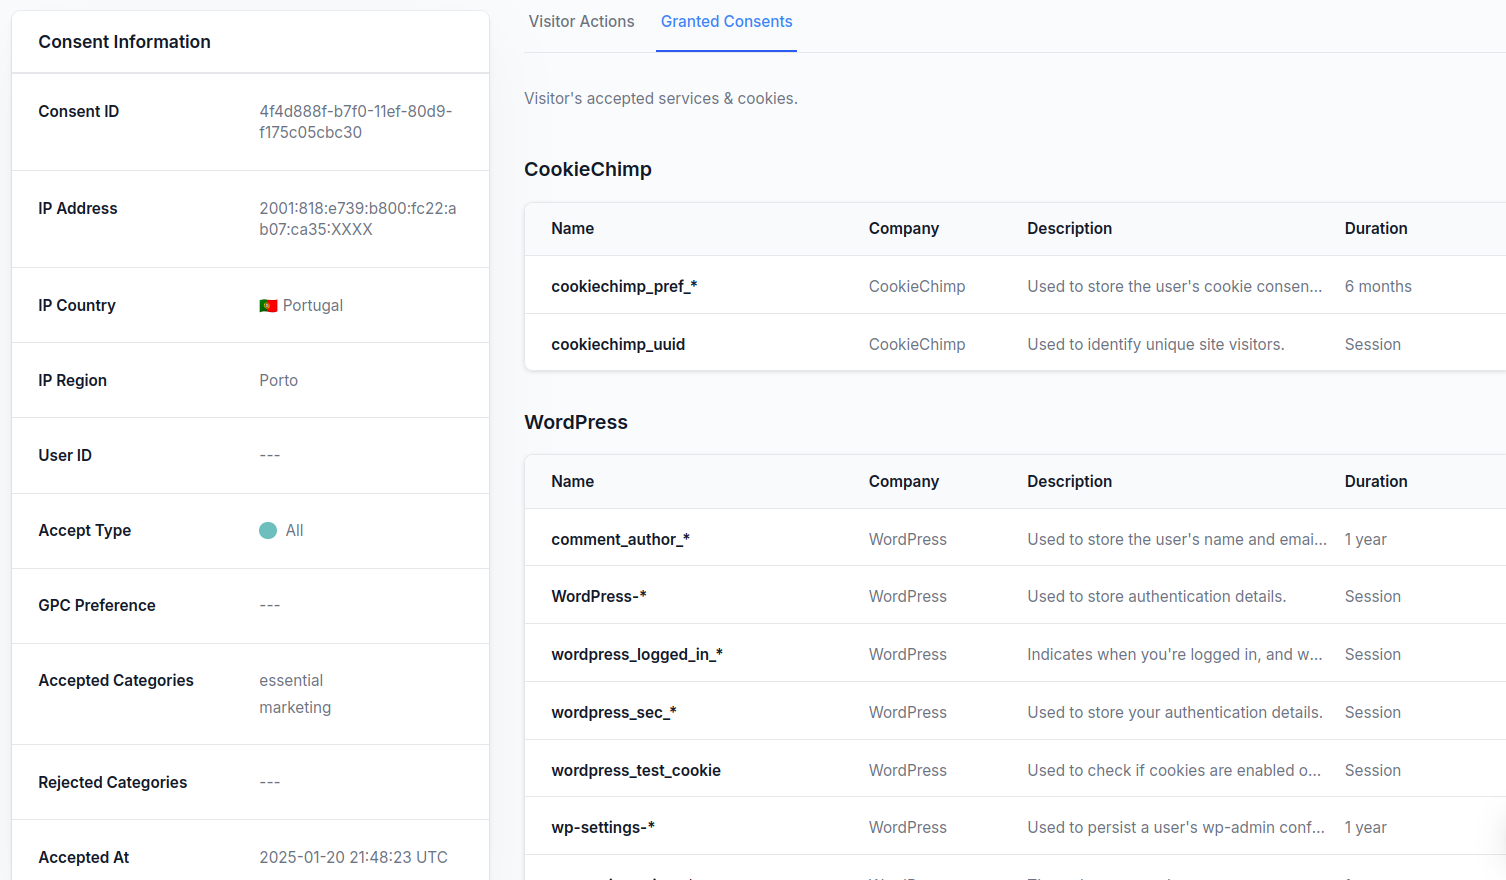
\includegraphics[width=1.0\textwidth]{images/consent.png}
    \end{center}
    \caption{Exemplo de visualização do consentimento na \textit{dashboard} do CookieChimp.}
\label{fig:dashboard-visualizacao}
\end{figure}

Desta forma, as \acrshort{cmp}s transmitem transparência e conformidade com as regulamentações de privacidade aos \textit{provedores de serviço}, e permitem que os utilizadores tenham escolha sobre os dados pessoais a partilhar.

\begin{figure}[h]
\begin{center}
	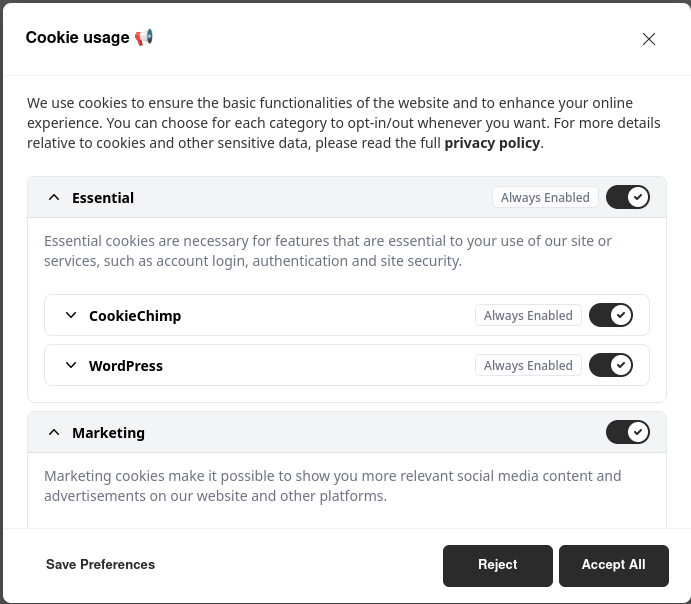
\includegraphics[width=1.0\textwidth]{images/banner.png}
\end{center}
\caption{Exemplo de banner de consentimento exibido ao utilizador.}
\label{fig:banner}
\end{figure}
% Tenho alguma duvida sobre a utilidade da figura

\newpage

\section{Plataformas e funcionalidades}
Entre as soluções encontra-se plataformas como Osano, Cookiebot, Tarteaucitron.js, Klaro.js e Consent Manager. Cada plataforma oferece funcionalidades específicas, mas têm em comum o foco na conformidade com as regulamentações de privacidade existentes.

\begin{itemize}
    \item Osano: Oferece uma interface intuitiva de personalização e um sistema eficiente de gestão de preferências, facilitadas por uma boa acessibilidade \cite{osano}. Inclui recursos avançados como armazenamento local de preferências, do lado do cliente, onde todo o acesso ao \textit{local storage} e aos \textit{cookies} (pequenos ficheiros de texto armazenados no navegador que guardam informações sobre as preferências e atividades do utilizador num site) feito pelo \textit{script} do Osano ocorre no contexto da página de execução e é tratado como \textit{cookie} de primeira parte. Isto significa que os dados do consentimento não são enviados a cada requisição, mas sim guardados localmente no \textit{browser}, utilizando o \textit{local storage} do navegador para armazenar dados auxiliares. Contudo, por ser uma solução proprietária, apresenta limitações na verificação do processamento de dados entre o navegador e o servidor, como por exemplo, opções limitadas de personalização, problemas de complexidade, exigindo suporte adicional para obter uma utilização mais eficaz para organizações de maiores dimensões e a gestão de cookies requer modificações extensas, tornando desafiador alcançar as funcionalidades desejadas.

    \item Cookiebot: Fornece uma solução robusta que analisa automaticamente até 10.000 páginas por domínio \cite{Cookiebot2024}. Implementa um sistema inteligente para detetar mudanças nos \textit{cookies} e rastreadores do website. O estado de consentimento do utilizador é armazenado localmente no navegador mediante um \textit{cookie}, denominado por \textit{CookieConsent}, que inclui um identificador único de consentimento (Consent ID) que se liga a um registo no servidor do Cookiebot para efeitos de auditoria da própria \acrshort{cmp} e prova legal. A principal limitação está na natureza fechada do código, que dificulta verificações independentes do funcionamento interno e a falta de possibilidade de auditoria do lado do cliente.

    \item Tarteaucitron.js \& Klaro.js: São soluções de código aberto que se destacam pela flexibilidade \cite{tarteaucitron}. Tarteaucitron.js permite extensões personalizadas e um carregamento otimizado de \textit{scripts} (fragmentos de código executados no navegador que permitem carregar funcionalidades externas, podendo recolher dados sobre a navegação do utilizador), armazenando as preferências de consentimento num \textit{cookie} do lado do cliente. Klaro.js oferece um sistema flexível de armazenamento de preferências e suporte a múltiplos idiomas, garantindo persistência local do lado do cliente sem necessidade de servidores externos. Ambos permitem personalização completa do controlo de \textit{cookies} e asseguram ser a ferramenta para estar em conformidade com os regulamentos impostos.

    \item Consent Manager: Permite sincronização instantânea das preferências do utilizador entre diferentes \textit{tabs} do navegador \cite{ConsentManager2024}. As preferências de consentimento são armazenadas localmente no navegador, assegurando a persistência das escolhas, sem necessidade de comunicação constante com o servidor. Embora ofereça recursos de gestão e uma integração eficiente, devido à sua natureza fechada, limita a transparência e dificulta a possibilidade de auditorias independentes de verificação do modo como os dados de consentimento são processados e como o sistema implementa o bloqueio e a transmissão de \textit{cookies} e rastreadores.

    \item CookieChimp: Destaca-se pela facilidade de integração com sistemas externos, como plataformas de análise, gestão de conteúdos e aplicações corporativas \cite{CookieChimp2024}. Disponibiliza uma \acrshort{api} RESTful, bem documentada, que permite a interoperabilidade com diferentes ambientes tecnológicos. A sua eficiência manifesta-se na capacidade de processar e sincronizar preferências de consentimento em tempo real, com baixo impacto no desempenho do website e elevada fiabilidade na atualização dos estados de consentimento.
\end{itemize}

Apesar dessas soluções estarem bem posicionadas para garantir a conformidade legal, um problema recorrente nas \acrshort{cmp}s existentes é a falta de visibilidade sobre os consentimentos transmitidos. Os utilizadores não sabem exatamente o que acontece com as suas informações durante a navegação, como os identificadores de sessão e preferências de consentimento, depois deste ser fornecido. Não existe uma forma clara e acessível para verificar se as escolhas feitas são efetivamente respeitadas, o que levanta questões sobre a transparência e a auditoria. Com isto em mente, nenhum dos \acrshort{cmp} oferece a possibilidade de o cliente poder demonstrar de forma independente as suas escolhas em termos de consentimento de uma maneira não repudiável e verificável, caso se torne evidente uma quebra do consentimento concedido.


\section{Limitações das \acrshort{cmp}s Existentes}

As \acrshort{cmp}s desempenham um papel crucial ao fornecer aos utilizadores uma forma de consentir explicitamente o uso dos seus dados pessoais. Entre as soluções, Osano, Cookiebot, Tarteaucitron.js, Klaro.js, Consent Manager e CookieChimp. Cada uma destas plataformas oferece funcionalidades específicas e foca-se na conformidade com regulamentos de privacidade, como o \acrshort{rgpd}. No entanto, apesar da sua importância, essas plataformas apresentam várias limitações que comprometem a transparência, a auditabilidade e a confiança no processamento de dados.

Para uma gestão de consentimento mais eficiente e alinhada com as expectativas dos utilizadores e as exigências regulamentares, certas características são fundamentais.
Por exemplo, a capacidade de uma auditoria do processo, garantindo que os utilizadores possam comprovar a confiabilidade da plataforma.
A auditabilidade é uma qualidade desejada, uma vez que possibilita aos utilizadores verificar se os seus pedidos são efetivamente respeitados, fornecendo uma camada adicional de confiança ao permitir a estes comprovar como as suas informações foram guardadas e processadas pelas entidades respetivas.
No entanto, as \acrshort{cmp}'s não oferecem, de forma nativa, mecanismos robustos de auditabilidade. Embora recolham e armazenem o consentimento dos utilizadores, raramente permitem verificar de forma transparente como esse consentimento foi processado, se foi cumprido ou se ocorreu alguma violação no seu tratamento.

A intuitividade da interface também é importante para garantir que os utilizadores consigam facilmente compreender e controlar as suas preferências de consentimento.
Complementarmente, a personalização das configurações de consentimento oferece maior flexibilidade, permitindo que as plataformas possam ser adaptadas a diferentes contextos organizacionais, respeitando as necessidades específicas de cada caso.
Por fim, a presença de uma \textit{API RESTful} permite que a \acrshort{cmp} se integre facilmente com outros sistemas, o que é particularmente relevante em ambientes mais complexos.

A tabela \ref{tab:cmp-caracteristicas} compara algumas das plataformas mais populares, destacando as suas capacidades em relação a estas características-chave e as suas limitações:

\label{tab:cmp-caracteristicas}
\begin{table}[H]
\centering
\caption{Comparação das principais características das \acrshort{cmp}s existentes}
\resizebox{\textwidth}{!}{%
\begin{tabular}{|l|c|c|c|c|c|c|}
\hline
\textbf{Característica} & \textbf{Osano} & \textbf{Cookiebot} & \textbf{Tarteaucitron.js} & \textbf{Klaro.js} & \textbf{Consent Manager} & \textbf{CookieChimp} \\ \hline
\textit{open-source}    &                &                     & X                          & X                &                           &                       \\ \hline
Auditabilidade          &                &                     &                            &                  &                           &                       \\ \hline
Intuitivo              & X              & X                   &   X                         &                 & X                         & X                     \\ \hline
Personalização         &                & X                   & X                          & X                &                           & X                     \\ \hline
RESTful API            &                & X                   &                            &                  & X                         & X                     \\ \hline
\end{tabular}%
}
\end{table}


\subsection{Discussão}

Além das limitações específicas de cada plataforma, existem problemas mais gerais que afetam as \acrshort{cmp}s tradicionais:

Primeiramente, verifica-se uma falta de transparência em como os dados dos utilizadores são processados e armazenados após o consentimento. Muitas plataformas não oferecem uma visão clara aos utilizadores, que frequentemente desconhecem se o consentimento foi transmitido corretamente ao servidor ou se as suas escolhas estão a ser respeitadas.

No domínio da gestão do consentimento, esta é também uma lacuna presente em praticamente todas as \acrshort{cmp}s. A maioria das plataformas oferece funcionalidades e estatísticas orientadas para o \textit{provedor de serviços}, mas do lado do utilizador não existe uma ferramenta que permita uma gestão eficiente dos consentimentos. Esta limitação impede o armazenamento e a consulta sistemática dos consentimentos estabelecidos entre ambas as entidades, comprometendo a transparência e o controlo efetivo por parte do utilizador.

Com isto, outra limitação crítica é a ausência de mecanismos robustos de confiança. As \acrshort{cmp}s existentes não permitem uma verificação em tempo real do cumprimento das escolhas do utilizador. Esta ausência torna difícil garantir que os dados recolhidos sejam processados de forma consistente com os regulamentos de privacidade, como o \acrshort{rgpd}.

Por fim, destaca-se o facto de que muitas soluções disponíveis no mercado são soluções fechadas. Isto significa que o código-fonte não está acessível ao público, impossibilitando auditorias independentes ou personalizações técnicas por terceiros. Este aspeto não limita apenas a flexibilidade técnica, mas reduz também a confiança geral nos processos internos das plataformas.

Embora estas \acrshort{cmp}s cumpram aspetos básicos de conformidade regulatória, tornam-se insuficientes para os desafios de gestão de consentimento. Assim, a criação de uma solução mais robusta, aberta e transparente surge como uma necessidade premente, capaz de superar essas limitações e estabelecer novos padrões de confiança no tratamento de dados pessoais.

\section{Mecanismos Criptográficos}

Mecanismos criptográficos constituem a base para a construção de sistemas de gestão de consentimento que sejam verificáveis, seguros e auditáveis. Estes mecanismos garantem propriedades essenciais como a autenticidade, integridade, confidencialidade e não repúdio, sendo fundamentais para assegurar que as ações dos utilizadores e das entidades envolvidas num processo de recolha e prova de consentimento possam ser validadas de forma independente.

No contexto da gestão de consentimento digital, a utilização destes mecanismos permite que as decisões de um utilizador, como aceitar ou rejeitar o tratamento dos seus dados, sejam registadas de forma verificável e não repudiável \citep{cryptoeprint:2024/1839}.

Neste âmbito, dois mecanismos destacam-se: as assinaturas digitais, que asseguram a integridade e autenticidade das declarações de consentimento, e os certificados digitais, que permitem estabelecer a identidade das partes envolvidas e criar um canal de confiança entre elas. Em conjunto, estes elementos possibilitam a criação de provas de consentimento digital que podem ser auditadas, validadas e utilizadas como evidência.

\subsection{Certificados digitais}

Os certificados desempenham um papel fundamental na garantia de identidade e na criação de comunicações seguras. De forma simplificada, um certificado digital é um ficheiro que associa uma chave pública a uma entidade (por exemplo, um utilizador ou um servidor). Esta associação é validada por uma \acrlong{ca} (\acrshort{ca}), que funciona como uma entidade de confiança responsável por emitir e assinar certificados.

A chave privada deve permanecer confidencial, pois é utilizada para operações críticas, como a criação de assinaturas digitais. Já a chave pública, incluída no certificado, pode ser partilhada e serve para validar essas assinaturas.

A \acrshort{ca} raiz (root \acrshort{ca}) é a autoridade de topo, responsável por assinar certificados de entidades intermédias ou diretamente de clientes e servidores. Esta última considera-se uma má prática, normas internacionais como a ETSI EN 319 411 \citep{ETSI_EN_319_411_1} proíbem explicitamente o uso direto da Root CA para emitir certificados operacionais. Este mecanismo hierárquico garante que, ao receber um certificado, é possível verificar a sua autenticidade através da cadeia de confiança estabelecida pela autoridade certificadora.

\subsection{Assinatura Digital}

A assinatura digital é um mecanismo criptográfico baseado em criptografia de chave pública, concebido para garantir a autenticidade e a integridade de uma mensagem ou documento eletrónico. O seu funcionamento baseia-se em dois elementos fundamentais: a chave privada e a chave pública. A chave privada é utilizada para gerar a assinatura digital e deve permanecer secreta, acessível apenas ao titular. A chave pública é distribuída, neste caso através de certificados digitais, permitindo que qualquer entidade verifique a validade da assinatura.

Desta forma, a assinatura digital assegura três propriedades essenciais \citep{digitalsignatures}:
\begin{itemize}
    \item \textbf{Autenticidade}: confirma que a mensagem foi assinada pela entidade detentora da chave privada correspondente.
    \item \textbf{Integridade}: garante que o conteúdo não foi alterado após a assinatura.
    \item \textbf{Não repúdio}: impede que o autor negue a sua participação no processo, tornando a assinatura uma evidência legalmente relevante.
\end{itemize}

As assinaturas digitais constituem o fundamento de sistemas confiáveis de registo de consentimentos, transações financeiras e documentos eletrónicos, sendo amplamente utilizadas em padrões de segurança e infraestruturas de chave pública.


\section{Gestão de consentimento baseada em \textit{{Blockchain}}}

Uma abordagem promissora para a auditoria de consentimento de dados é a utilização de \textit{blockchain} e contratos inteligentes. Esta tecnologia distingue-se por características como descentralização, transparência, integridade e imutabilidade, proporcionando um registo distribuído e resistente a alterações não autorizadas. Assim, pode ser utilizada para documentar de forma segura e auditável todas as interações relacionadas com o consentimento dos utilizadores. Os contratos inteligentes, por sua vez, podem permitir automatizar a verificação e aplicação das condições definidas, garantindo que os dados são partilhados ou processados apenas de acordo com as permissões concedidas, de forma autónoma e transparente.

O conceito de \textit{blockchain} foi inicialmente popularizado com o surgimento do Bitcoin \citep{nakamoto2008bitcoin}, a primeira criptomoeda descentralizada. O Bitcoin utiliza \textit{blockchain} como um livro-razão público e imutável, onde todas as transações são registadas de forma segura e verificável sem a necessidade de uma entidade central. Com o tempo, novas aplicações da tecnologia \textit{blockchain} emergiram, indo além das criptomoedas e incluindo domínios como gestão de identidade digital, rastreamento de cadeias de fornecimento e, mais recentemente, gestão de consentimento de dados.

Além do Bitcoin, outro marco importante na evolução da tecnologia \textit{blockchain} foi o surgimento da Ethereum \citep{buterin2014next}, que introduziu a capacidade de executar contratos inteligentes. Diferente do Bitcoin, cujo foco principal é a transferência segura de valor, a Ethereum foi projetada para suportar aplicações descentralizadas através de contratos inteligentes, permitindo que regras e condições predefinidas sejam automaticamente executadas sem necessidade de intermediários. Essas capacidades tornaram a Ethereum uma das principais plataformas para aplicações \textit{blockchain}, incluindo soluções para gestão de consentimento de dados baseadas em contratos inteligentes \citep{Frank2018}.

Nos últimos anos, investigadores têm proposto diferentes abordagens baseadas no uso de contratos inteligentes e na tecnologia \textit{blockchain}, que oferecem características desejáveis, como transparência, rastreabilidade, não-repúdio e imutabilidade. Essas propostas podem ser classificadas de acordo com dois principais cenários:

\begin{itemize}
    \item Consentimento gerido pelo titular: Quando um utilizador tem autonomia e deseja partilhar os seus dados pessoais com terceiros, mantendo o controlo total sobre as permissões concedidas e podendo revogá-las a qualquer momento \citep{Merlec2021}.
    \item Consentimento gerido por terceiros: Quando um fornecedor de serviços recolhe dados pessoais de um utilizador para posterior processamento, normalmente como parte da utilização de um produto ou serviço, sendo necessário garantir a conformidade com as regras definidas pelo utilizador e pelas regulamentações em vigor. Nesse caso, plataformas centralizadas em blockchain atuam como controladores do consentimento \citep{Aldred2019}.
\end{itemize}

Atualmente, já existem várias plataformas que utilizam \textit{blockchain} para gestão de consentimento. 
As soluções analisadas a seguir são exemplos de consentimento gerido diretamente pelo titular dos dados.

\begin{itemize}
    \item GDPR-Compliant Personal Data Management: Uma solução baseada em \textit{blockchain} proposta por \citep{nguyen2020gdpr}, que garante a conformidade com o \acrshort{rgpd} através de dois sistemas de registo distribuídos. O sistema implementa o controlo de acesso através de um modelo de identidade complexa (c-ID) que combina chaves assimétricas do \acrshort{ds} e \acrshort{dc}, juntamente com referências encriptadas aos dados (\textit{data\_pointer}). A solução utiliza \textit{smart contracts} específicos (\textit{GrantConsent, RevokeConsent e DataAccess}) para regular o ciclo de vida do consentimento, mantendo um registo imutável das operações no \textit{log\_ledger} enquanto as políticas de acesso e referências aos dados são armazenadas no \textit{3A\_ledger}. Esta implementação em \textit{Hyperledger Fabric} assegura não só o registo descentralizado do consentimento, mas também a sua validação contínua e auditável.

    \item Privacy by \textit{blockchain Design}: Uma abordagem proposta por \citep{wirth2018privacy} que foca no registo e verificação do consentimento através da \textit{blockchain}. O sistema utiliza \textit{smart contracts} especializados para gerir o ciclo de vida do consentimento, permitindo que os dados pessoais sejam armazenados \textit{off-chain} enquanto a \textit{blockchain} mantém apenas \textit{hashes} e ponteiros criptográficos dos dados (\textit{data\_pointer}). A solução implementa uma arquitetura que permite que o \textit{titular dos dados} seja notificado sempre que os seus dados são acedidos, através de um contrato inteligente que verifica a validade dos pedidos de acesso e regista todas as operações de forma transparente. Desta forma, o sistema garante que o consentimento é dado de forma específica e verificável para cada caso de uso, em vez de ser baseado em cláusulas abstratas predefinidas.
\end{itemize}

Entre os benefícios da utilização de \textit{blockchain} na gestão de consentimento, destacam-se:

\begin{itemize}
    \item Transparência e Imutabilidade: Em \textit{blockchains} públicas, o registo de consentimentos é transparente, permitindo que qualquer participante verifique as transações, enquanto a estrutura imutável garante que os dados não possam ser alterados ou manipulados após serem armazenados.
    \item Automatização: Os contratos inteligentes podem ser configurados para permitir ou restringir o acesso aos dados com base nos consentimentos fornecidos, assegurando que as regras do \acrshort{rgpd} sejam respeitadas automaticamente.
    \item Auditabilidade: Qualquer alteração nos consentimentos pode ser rastreada, permitindo a verificação da conformidade com a regulamentação e aumentando a confiança dos utilizadores.
    \item Descentralização: A ausência de uma autoridade central única e a validação por múltiplos participantes reduzem o risco de manipulação dos consentimentos, aumentando a integridade e a confiança nos dados.
    \item Não Repúdio: Uma vez registado um consentimento no \textit{blockchain}, ele não pode ser repudiado ou modificado de forma fraudulenta, garantindo que todas as partes envolvidas possam verificar e comprovar a autenticidade do registo.
\end{itemize}

No entanto, a blockchain apresenta também algumas desvantagens. Um dos principais desafios associados à utilização da \textit{blockchain} na gestão de consentimento decorre precisamente da sua transparência. Os desenvolvedores têm de considerar cuidadosamente os inconvenientes de tornar toda a informação acessível publicamente e encontrar soluções que permitam proteger os dados sensíveis. Por exemplo, dependendo da forma como este registo é armazenado, é possível rastrear os serviços que um utilizador visita, permitindo inferir os seus interesses pessoais. Para mitigar este risco, seria necessária a inclusão de uma camada criptográfica adicional, de modo a preservar o anonimato e assegurar que os dados sensíveis permanecem privados, sem comprometer a transparência e a integridade do sistema.
Outro desafio associado em aplicações como a gestão de consentimento, prende-se com a eficiência e os custos. Cada transação não é processada por uma única unidade, mas por toda a rede, o que implica uma repetição massiva das operações e um custo significativamente superior ao de sistemas tradicionais. Para além disso, o tempo de resposta da rede é limitada pelos mecanismos de consenso, que tendem a criar um \textit{trade-off} entre descentralização e rapidez. Adicionalmente, a introdução de aplicações baseadas em \textit{blockchain} enfrenta barreiras regulatórias e legais, nomeadamente quanto à validade e enquadramento dos \textit{smart contracts}. Estes fatores devem ser ponderados cuidadosamente, de modo a justificar o valor acrescentado da tecnologia face às suas limitações operacionais e jurídicas.

Apesar de tudo, o uso de \textit{blockchain} na gestão de consentimento representa uma abordagem inovadora que pode aumentar a confiança e garantir maior transparência no tratamento de dados pessoais.

 

\section{Síntese do capítulo} 

Neste capítulo são analisadas as principais soluções existentes para a gestão de consentimento, com destaque para as \acrshort{cmp}s mais utilizadas no mercado. Verificou-se que, embora estas plataformas respondam às exigências básicas de conformidade com o \acrshort{rgpd}, persistem limitações significativas relacionadas com transparência, auditabilidade e abertura do código. Foram ainda discutidas abordagens complementares, nomeadamente o recurso a tecnologias como \textit{blockchain} e contratos inteligentes, que procuram colmatar algumas destas falhas e introduzir novos níveis de confiança e verificabilidade no tratamento de dados pessoais.

A constatação destas limitações motiva o desenvolvimento de uma solução alternativa que combine a flexibilidade das \acrshort{cmp}s existentes com mecanismos robustos de transparência e auditoria. No capítulo seguinte é apresentada a solução proposta, concebida de forma genérica e modular, capaz de responder a estes desafios e de servir como base para a implementação de soluções concretas de gestão de consentimento.
